\section{Техническое задание}
\subsection{Основание для разработки}

Полное наименование системы: "<Маркетплейс для реализации цифровых предметов внутри игры «Stay Out»">.

Основанием для разработки программы является приказ ректора ЮЗГУ от «07» апреля 2023 г. №1620-с «Об утверждении тем выпускных квалификационных работ».

\subsection{Цель и назначение разработки}

Основное назначение разработки маркетплейса для реализации цифровых предметов внутри игры «Stay Out» заключается в создании интегрированной платформы, которая обеспечит удобный и безопасный способ обмена, покупки и продажи внутриигровых предметов. Маркетплейс призван решать несколько ключевых задач:

\subsubsection{Удовлетворение потребностей игроков}
Маркетплейс предоставляет игрокам возможность легко покупать, продавать и обменивать цифровые предметы, такие как оружие, скины, внутриигровая валюта и другие уникальные объекты. Это позволяет игрокам разнообразить игровой процесс, улучшать свои игровые персонажи и получать больше удовольствия от игры.

\subsubsection{Увеличение вовлеченности и удержания игроков}
Интеграция маркетплейса стимулирует игроков проводить больше времени в игре, так как они получают дополнительные возможности для взаимодействия и торговли. Это способствует увеличению вовлеченности и удержания игроков, что в конечном итоге повышает популярность и доходность игры.

\subsubsection{Создание устойчивой игровой экономики}
Маркетплейс способствует формированию устойчивой игровой экономики, где игроки могут зарабатывать внутриигровую валюту и ресурсы, продавая свои предметы другим игрокам. Это создает динамичную и самоподдерживающуюся экосистему, которая улучшает общий игровой опыт и делает игру более интересной и реалистичной.

\subsubsection{Обеспечение безопасности транзакций}
Одной из ключевых задач разработки маркетплейса является обеспечение безопасности всех транзакций. Это включает в себя защиту данных пользователей, предотвращение мошенничества и обеспечение прозрачности всех операций. Надежные механизмы безопасности повышают доверие игроков к платформе и делают процесс торговли безопасным и надежным.

\subsubsection{Создание новых источников дохода для разработчиков}
Маркетплейс открывает новые возможности для монетизации игры, предоставляя разработчикам дополнительные источники дохода. Это может включать комиссионные с продаж, платные подписки для доступа к эксклюзивным предметам и другие модели дохода. Таким образом, маркетплейс помогает разработчикам инвестировать в дальнейшее развитие и улучшение игры.

\subsubsection{Улучшение взаимодействия внутри игрового сообщества}
Маркетплейс способствует улучшению взаимодействия между игроками, создавая платформу для обмена и торговли. Это помогает формировать более тесное и активное сообщество, где игроки могут делиться своими достижениями и получать поддержку от других участников.

В заключение, разработка маркетплейса для игры «Stay Out» направлена на создание удобного, безопасного и функционального инструмента для торговли цифровыми предметами, который будет способствовать развитию игровой экономики, увеличению вовлеченности игроков и созданию новых возможностей для монетизации игры.


\subsection{Требованияк программной системе}

\subsubsection{Требования к данным программной системы}

Концептуальная модель данных программной системы представлена на рисунке ~\ref{fig:modelbd}.

\begin{figure}[h]
	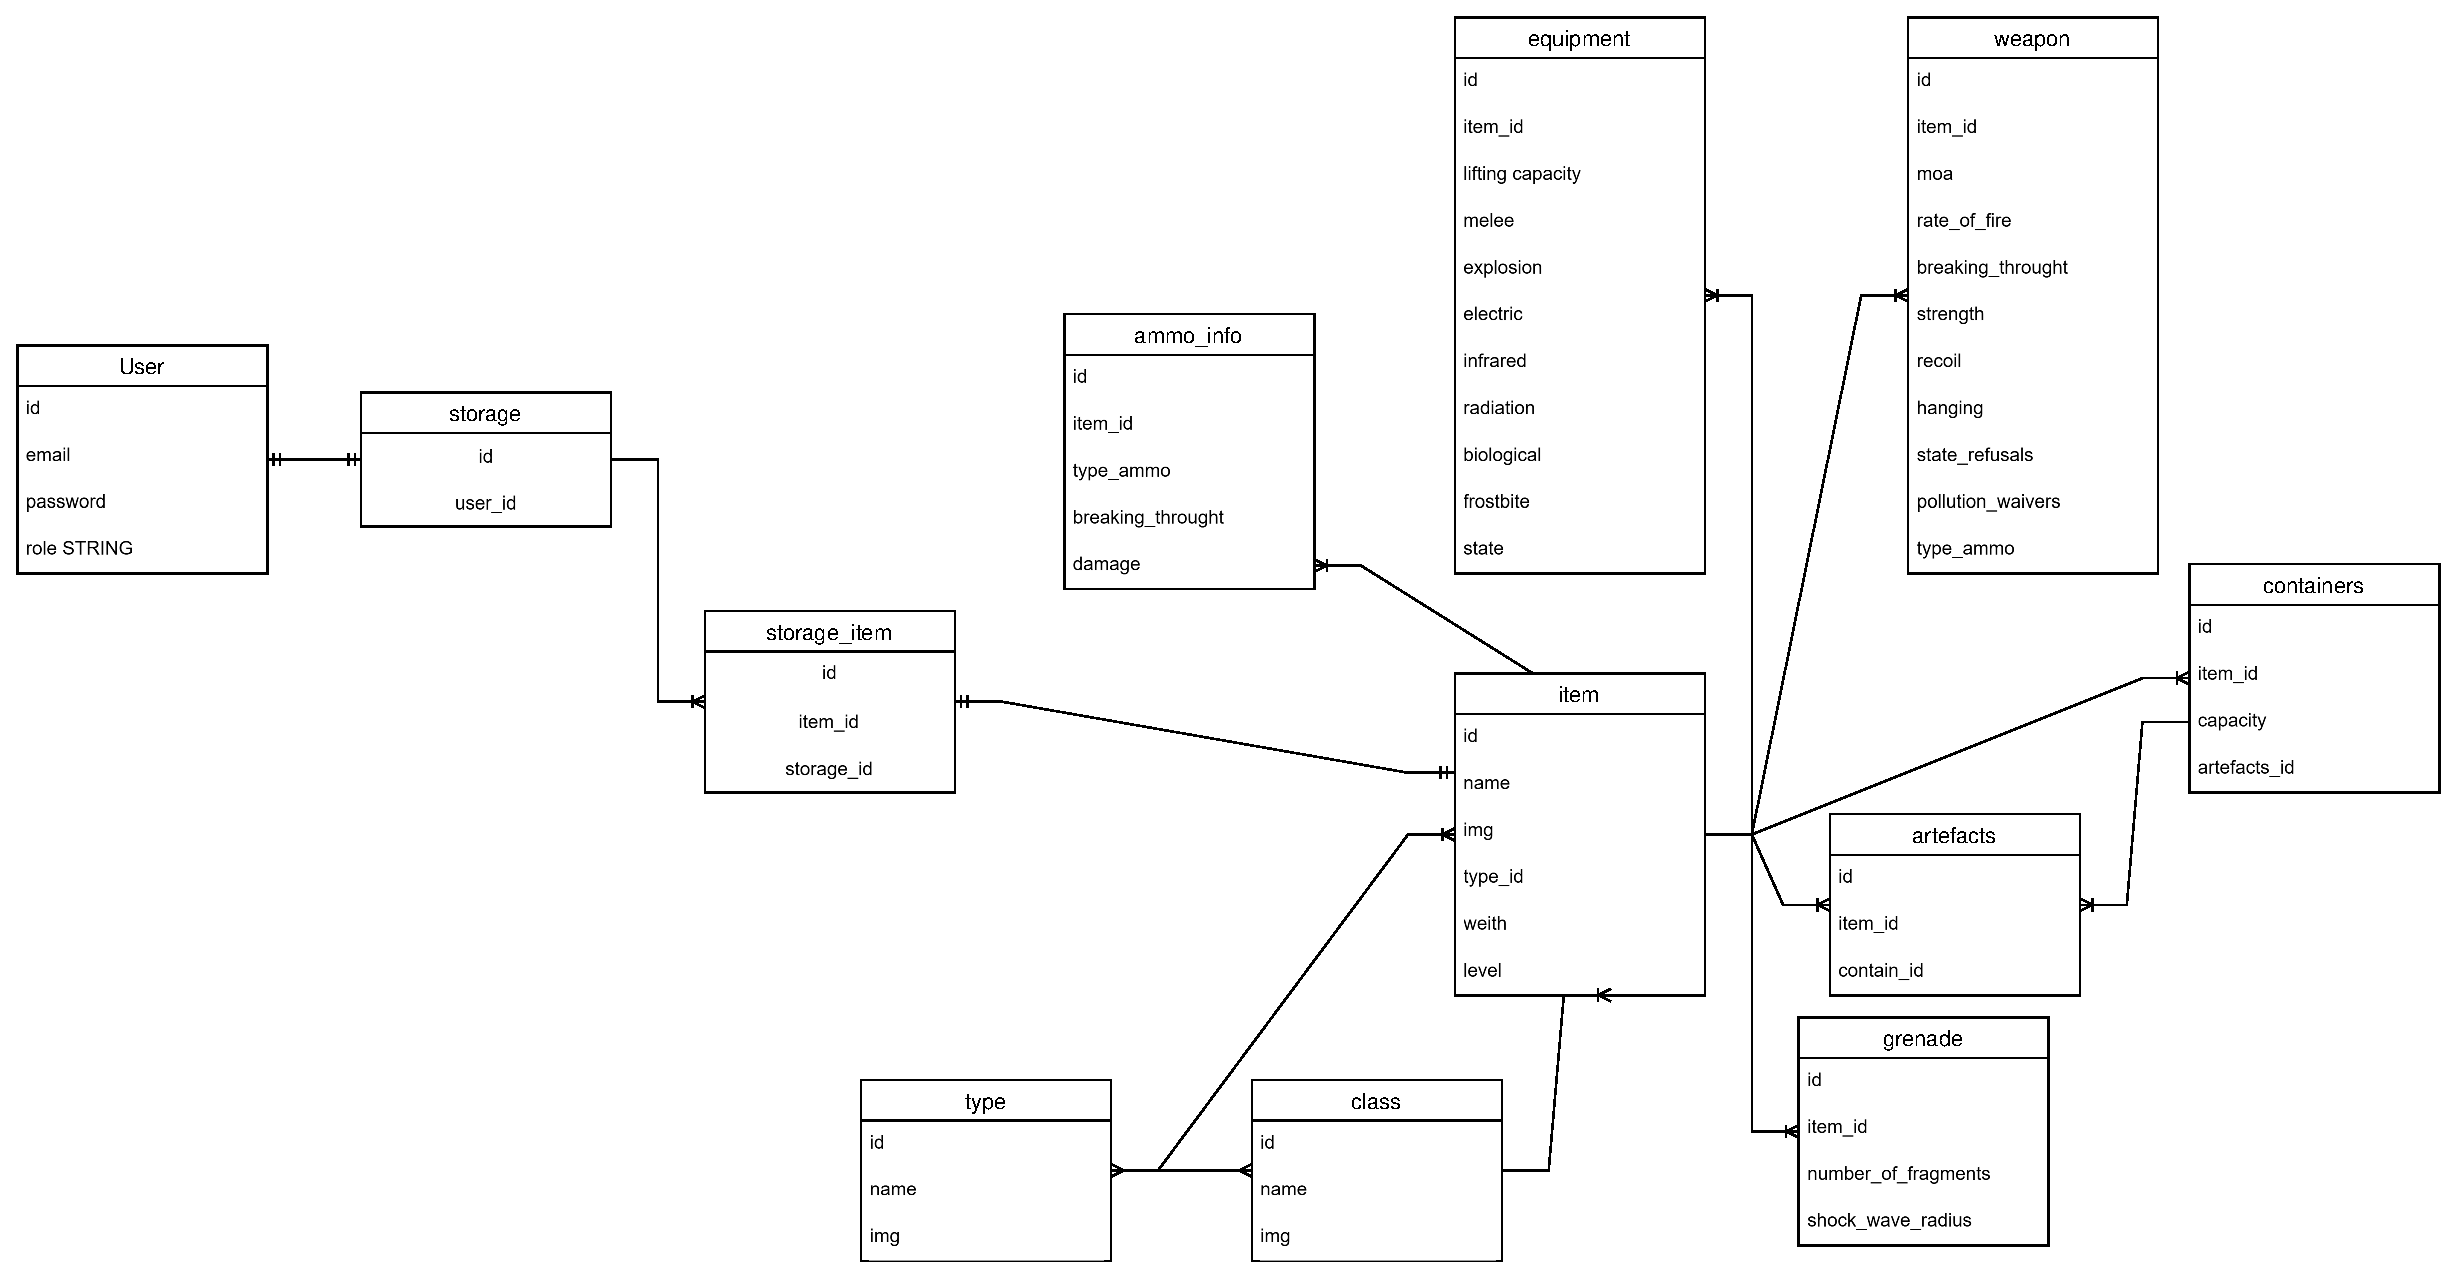
\includegraphics[width=1\linewidth]{images/modelbd}
	\caption{Концептуальная диаграмма "сущность-связь"}
	\label{fig:modelbd}
\end{figure}
%\vspace{-\figureaboveskip} % двойной отступ не нужен (можно использовать, если раздел заканчивается картинкой)

Система должна поддерживать добавление и редактирование характеристик оружия, снаряжения, боеприпасов и других категорий предметов. Также она должна обеспечивать возможность быстрого редактирования существующих предметов для отображения актуальной информации о товарах.

\subsubsection{Функциональные требования к программной системе}

В разрабатываемой программной системе должны быть реализованы следующие функции:

\begin{enumerate}
	\item Регистрация и аутентификация пользователей.
	\item Выбор сервера для торговли.
	\item Просмотр ассортимента.
	\item Просмотр информации об аккаунте.
	\item Администрирование системы.
\end{enumerate}

Диаграмма прецедентов представлена на рисунке ~\ref{fig:precendent}.

\begin{figure}[h]
	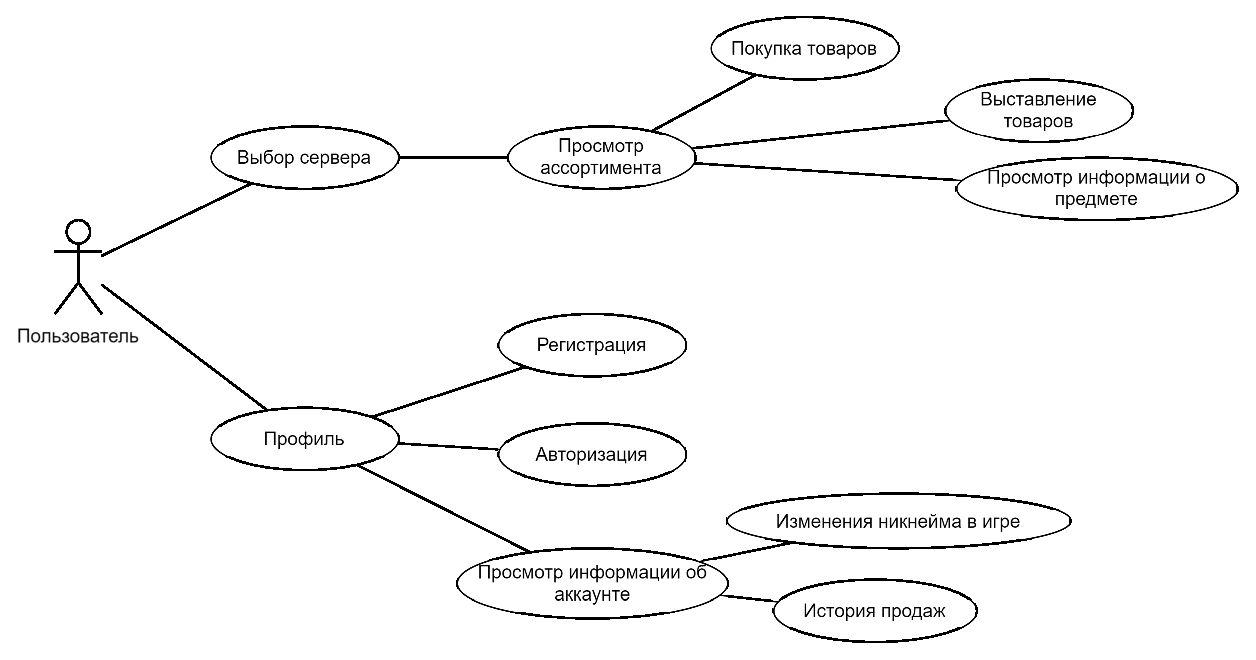
\includegraphics[width=1\linewidth]{images/precendent}
	\caption{Диаграмма прецедентов}
	\label{fig:precendent}
\end{figure}

\paragraph{Вариант использования «Выбор сервера»}

Заинтересованные лица и их требования: пользователь желает начать производить какие-либо действия на сайте, связанные с торговлей. Предусловие: открыта главная страница сайта. Постусловие: открывается нужная страница в соответствие с выбранным сервером. Основной успешный сценарий:

\begin{enumerate}
	\item Пользователь нажимает на кнопку выбора сервера на главной странице сайта.
	\item На сайте открывается модальное окно с доступными серверами.
	\item Пользователь выбирает нужный ему сервер.
	\item Приложение открывает страницу, соответствующую выбранному серверу.
\end{enumerate}

\paragraph{Вариант использования «Просмотр информации о товаре»}

Заинтересованные лица и их требования: пользователь желает получить больше информации о конкретном товаре. Предусловие: открыта страница какого-либо сервера. Постусловие: появляется модальное окно с полной информацией о товаре. Основной успешный сценарий:

\begin{enumerate}
	\item Пользователь нажимает на значок с изображением нужного товара.
	\item Приложение получает уникальный id предмета и отправляет запрос на сервер.
	\item Сервер формирует запрос в базу данных и передает данные в приложение.
	\item Приложение получает информацию от сервера и заполняет модальное окно в соответствие с полученной информацией.
\end{enumerate}

\paragraph{Вариант использования «Покупка товара»}

Заинтересованные лица и их требования: пользователь увидел интересующий его товар и захотел его приобрести. Предусловие: открыта страница какого-либо сервер. Постусловие: появляется уникальное сообщение, которое нужно скопировать и вставить в игре. Основной успешный сценарий:

\begin{enumerate}
	\item Пользователь нажимает на кнопку «Купить».
	\item  Приложение генерирует уникальное сообщение в соответствие с названием товаров и игровым никнеймом пользователя.
\end{enumerate}

\paragraph{Вариант использования «Регистрация»}

Заинтересованные лица и их требования: пользователь хочет создать свой аккаунт на сайте. Предусловие: пользователь еще не авторизовался на сайте. Постусловие: регистрация произведена, появляется значек с изображение профиля. Основной успешный сценарий:

\begin{enumerate}
	\item Пользователь нажимает на кнопку «Регистрация».
	\item Открывается экран регистрации пользователя.
	\item Пользователь вводит почту, логин, пароль и повторный пароль.
	\item Приложение отправляет запрос на сервер.
	\item Сервер формирует запрос в базу данных на создание аккаунта.
	\item Если аккаунта с таким же логином или почтой не существует, создается новый аккаунт.
	\item Сервер передает информацию в приложение о результате создания аккаунта.
	\item Приложение открывает окно пользователю с результатами регистрации.
\end{enumerate}

\paragraph{Вариант использования «Авторизация»}

Заинтересованные лица и их требования: пользователь хочет войти в свой аккаунт на сайте. Предусловие: пользователь еще не авторизовался на сайте. Постусловие: авторизация произведена, появляется значок с изображение профиля. Основной успешный сценарий:

\begin{enumerate}
	\item Пользователь нажимает на кнопку «Авторизация».
	\item Открывается экран авторизации пользователя.
	\item Пользователь вводит почту, логин, пароль и повторный пароль.
	\item Приложение отправляет запрос на сервер.
	\item Сервер формирует запрос в базу данных.
	\item База данных возвращает результат о совпадении логина и пароля.
	\item Сервер передает информацию в приложение о результате авторизации.
	\item Приложение открывает окно пользователю с результатами авторизации.
\end{enumerate}

\paragraph{Вариант использования «Выставление товара»}

Заинтересованные лица и их требования: пользователь хочет продать какую-либо вещь. Предусловие: пользователь выбрал сервер и авторизовался. Постусловие: предмет добавляется в ленту товаров:

\begin{enumerate}
	\item Пользователь нажимает на элемент интерфейса (значок с изображением плюса).
	\item Приложение открывает модальное окно с полями ввода.
	\item Пользователь вводит название предмета полностью или его часть.
	\item Приложение выводит все совпадения.
	\item Пользователь выбирает нужный ему предмет.
	\item Приложение отправляет запрос на сервер.
	\item Сервер формирует запрос в базу данных на получения все характеристик предмета.
	\item Сервер передает данные в приложение.
	\item Приложение заполняет необходимые данные в соответствие с данными.
	\item Пользователь вводит недостающие данные и выставляет предмет на продажу.
	\item Приложение отправляет запрос на сервер.
	\item Сервер вносит данные в базу данных.
	\item Сервер передает информацию о результате приложению.
	\item Приложение оповещает пользователя об успехе выставления предмета на продажу.
\end{enumerate}

\paragraph{Вариант использования «Изменение пароля»}

Заинтересованные лица и их требования: пользователь хочет поменять свой пароль на аккаунте. Предусловие: пользователь авторизировался. Постусловие: изменение пароля:

\begin{enumerate}
	\item Пользователь нажимает на кнопку "Изменить пароль"
	\item Приложение открывает модальное окно с полями ввода.
	\item Пользователь вводит текущий пароль, новый пароль повторный новый пароль.
	\item Приложение отправляет запрос на сервер.
	\item Сервер формирует запрос в базу данных на смену пароля.
	\item Сервер передает данные в приложение.
	\item Приложение оповещает пользователя об успехе выставления предмета на продажу.
\end{enumerate}

\subsubsection{Требования пользователя к интерфейсу приложения}

На сайте должны быть реализованы следующие страницы:

\begin{enumerate}
	\item Страница «Выбор сервера» -- главная страница при открытии сайта, где отображается основной текст и возможность выбрать основной сервер для торговли.
	\item Страница «Лента товаров» -- страница, на которой отображаются все товары, выставленные другими пользователями в рамках выбранного сервера в соответствии с установленными параметрами фильтрации.
	\item Страница «Профиль» -- страница для просмотра и изменения данных аккаунта.
	\item Страница «Аутентификация» -- страница, на которой пользователь может создать новый аккаунт или зайти уже в существующий.
	\item Страница «Админ панель» - страница для особой категории пользователей, являющихся администраторами на сайте, для удобного добавления новых типов, классов и предметов.
	\item Страница «Ваши товары» -- страница, на которой отображаются все товары, выставленные авторизованным пользователем, позволяет изменять состояние предмета, будь то удаление, добавление или изменение.
	\item Страница «Информация о товаре» -- страница, на которой отображается информация о выбранном товаре.
\end{enumerate}

Помимо перечисленных страниц, на сайте должны быть реализованы следующие компоненты:

\begin{itemize}
	\item окно изменения пароля;
	\item окно создания классов;
	\item окно созадния типов;
	\item окно создания предметов;
	\item окно выбора серверов;
\end{itemize}

\subsubsection{Нефункциональные требования к программной системе}

\paragraph{Требования к надежности}

В процессе использования маркетплейса могут произойти различные аварийные ситуации. Для обеспечения устойчивости и защиты данных сайт должен соответствовать следующим требованиям:

\begin{itemize}
	\item система должна работать безотказно и минимизировать время простоя;
	\item система должна быть устойчивой к аппаратным и программным сбоям;
	\item обеспечение устойчивости системы при большом количестве одновременно активных сессий пользователей;
	\item обновления системы не должны нарушать работу существующих функций и данных.
\end{itemize}

\paragraph{Требования к безопасности}

Безопасность пользователя и его данных является очень важным фактом. Для обеспечения безопасного использования необходимо учитывать следующие требования к безопасности:

\begin{itemize}
	\item пароли пользователей должны храниться в зашифрованном виде, используя современные методы хеширования;
	\item регулярное обновление программного обеспечения для устранения известных уязвимостей;
	\item регулярное создание резервных копий всех критических данных и их безопасное хранение;
	\item предоставление пользователям рекомендаций и напоминаний по обеспечению безопасности их учетных записей;
	\item обеспечение быстрого оповещения пользователей и администраторов о возможных инцидентах.
\end{itemize}

\subsection{ Требования к программному обеспечению}

Для реализации программной системы должны быть использованы следующие языки программирования:

\begin{itemize}
	\item JavaScript - серверная часть приложения;
	\item JavaScript - клиентская часть приложения;
	\item SQL для запросов к базе данных.
	\item Рабочий проект.
\end{itemize}

Для доступа к клиентской части требуется веб-браузер с поддержкой
JavaScript стандарта ECMAScript 2015.

\subsection{Требования к оформлению документации}

Требования к стадиям разработки программ и программной документации для вычислительных машин, комплексов и систем независимо от их назначения и области применения, этапам и содержанию работ устанавливаются ГОСТ 19.102–77 и ГОСТ 34.601-90.

Программная документация должна включать в себя:

\begin{itemize}
	\item Анализ предметной области.
	\item Техническое задание.
	\item Технический проект.
	\item Рабочий проект.
\end{itemize}
